% portail-ajout-groupe.tex
\section{Ajouter un groupe à son profil}

\subsection{Affichage de tous les groupes disponibles}
Une fois l'onglet \og~\bsc{groupes}~\fg{} sélectionné comme le montre la capture d'écran la liste des groupes disponibles, 193 ici au message \textbf{Explorer les groupes (193)}. 
À sa droite une loupe vous permet de saisir un mot clé du nom du groupe si vous le connaissez et le filtre agira en affichant uniquement les éléments concernés.
\begin{figure}
	\centering
	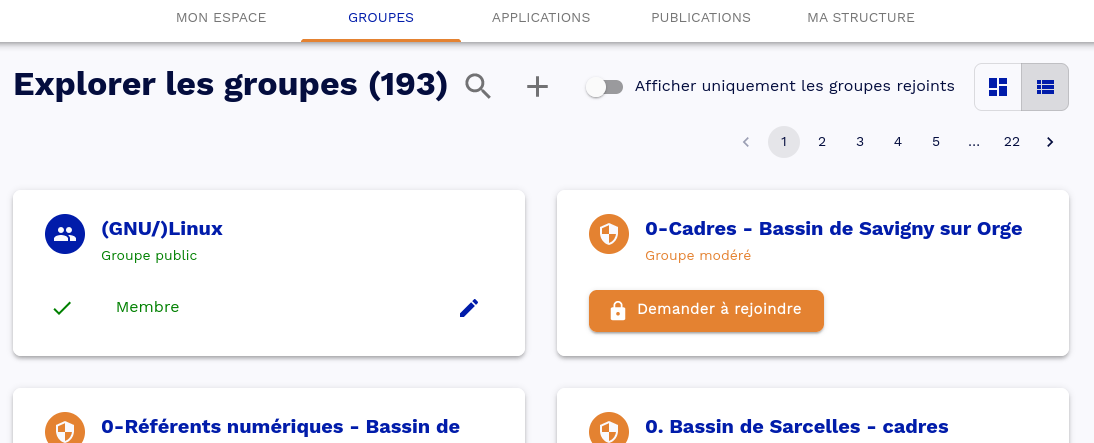
\includegraphics{./Captures/portail.groupes.selection.png}
	\caption{Affichage des différents groupes disponibles}
\end{figure}

À la droite de la loupe, un grand signe plus vous permet de créer un groupe, où, par défaut en tant que créateur, vous serez aussi l'administrateur.

\begin{quote}
	\emph{Là où l’on trouve un grand pouvoir, on trouve une grande responsabilité.}\newline
	\begin{flushright} Winston Churchill (1906) \end{flushright}
\end{quote}


\subsection{S'inscrire à un groupe}
Parmi les groupes se trouvent des groupes publics ouverts à tous, donc les accentuations colorées sont bleu où l'inscription est automatique dès que vous cliquez sur le bouton \fbox{$\boxed{\rightarrow}$ \hspace{0.1cm} Rejoindre le groupe}
\begin{figure}
	\centering
	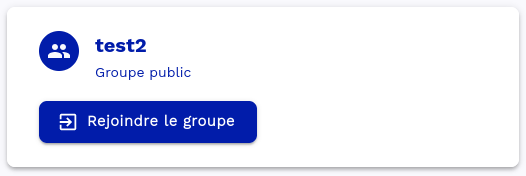
\includegraphics[width=0.500\linewidth]{Captures/portail.groupe.exemple.public.png}
	\caption{Exemple de groupe public}
\end{figure}
C'est le cas de ce groupe Test2 ou bien auparavant du groupe \textbf{(GNU)/Linux}, mais se trouvent aussi des groupes modérés à inscription suite à une validation, ces groupes apparaissent avec des icônes oranges circulaires représentant l'équivalent d'un bouclier, et aussi par une coloration orange. 
De même le bouton n'affiche pas \emph{Rejoindre le groupe} comme auparavant mais un cadenas et \textbf{Demander à rejoindre} puisqu'un modérateur ou un administrateur devra accepter l'inscription pour pouvoir accéder au groupe.

Si un icône a été défini pour le groupe, alors la coloration bleuté restera et l'icône du groupe s'affichera avec un icône générique (bleu ou orange) à ses côtés

\begin{figure}
	\centering
	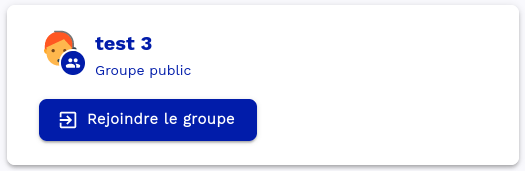
\includegraphics[width=0.500\linewidth]{./Captures/portail.groupe.exemple.public.avec.icone.png}
	\caption{Exemple de groupe public avec icône spécifique.}
\end{figure}

Il en va de même avec les groupes modérés évidemment.

une fois les groupes intéressants ajoutés au profil, ce dernier les affichera directement dans la zone ``\textbf{Mes groupes}'' dédiée aux groupes comme le montre la capture suivante.

\begin{figure}
	\centering
	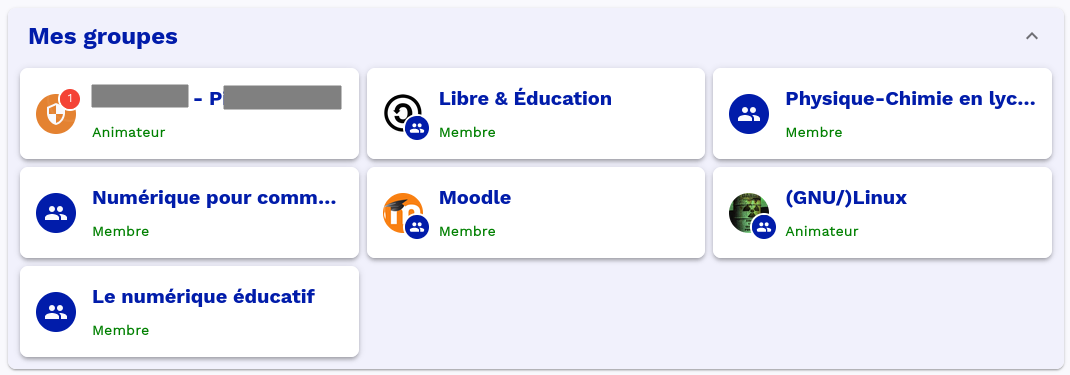
\includegraphics{./Captures/portail.accueil.mes.groupes.png}
	\caption{Les groupes ajoutés à mon profil.}
\end{figure}

Vous aurez noté sur le groupe du haut, à gauche, la présence d'un 1 dans un cercle rouge. 
Dans ce groupe modéré puisque de couleur orange où je suis animateur --comprendre administrateur-- il y a une notification. 
En l'occurrence il s'agit ...

\paragraph{Notez la présence d'un \^{} en haut à droite.}
Celui-ci permet de replier la zone consacrée à l'affichage de mes groupes.

\subsection{Gérer mes groupes}
La gestion des groupes s'effectue à partir du menu du profil. 
Bien évidemment, il s'agit de gérer les groupes dont on est administrateur ou modérateur, pas simple utilisateur
\begin{figure}
	\centering
	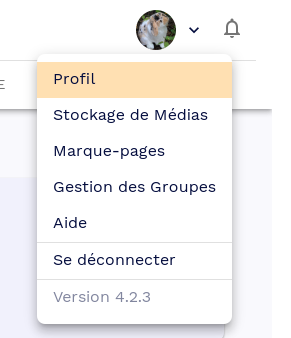
\includegraphics[width=0.3333\linewidth]{./Captures/menu.profil.png}
%	\caption{}
\end{figure}

\subsection{Détails d'un groupe}
En cliquant sur un des groupes, au hasard un de ceux administrés, voici les détails qui s'affichent. 
Ce tableau de bord complet montre tous les réglages et les options auxquelles il est possible d'accéder.
\begin{figure}
	\centering
	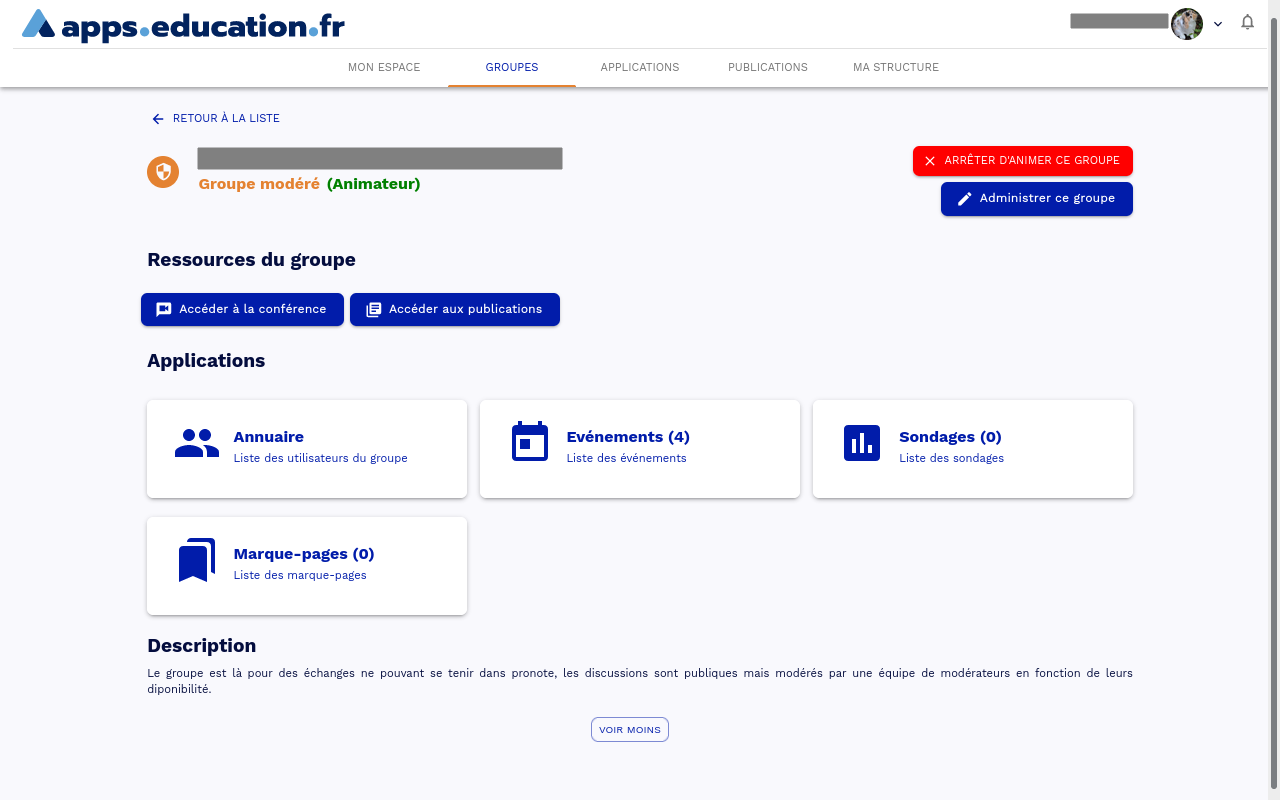
\includegraphics{./Captures/portail.groupe.affichage.details.png}
	\caption{L'intégralité des détails d'un groupe.}
\end{figure}
